\documentclass{article}
\usepackage{fullpage}
\usepackage{graphicx}
\usepackage{grffile}
\usepackage{caption}
\usepackage{subcaption}
\usepackage[margin=0.5in]{geometry}
\usepackage{float}
\graphicspath{
{/home/pannnnn/CSC320-A3/CS320/A3/test_images/}
}

% convert tif into png
\usepackage{epstopdf}
\epstopdfDeclareGraphicsRule{.tif}{png}{.png}{convert #1 \OutputFile}
\AppendGraphicsExtensions{.tif}

% make figure appear on top
\makeatletter
\setlength{\@fptop}{0pt}
\makeatother

\begin{document}

\noindent
University of Toronto\\
{\sc CSC}320, Mar 28th, 2017\\[10pt]
{\LARGE\bf Assignment 3: Yuhui Pan - 1001239395 - panyuhui} \\[10pt]

%----------------------------------------------------------------------------------------------------------------------
\section*{Part2: Report \& Experimental evaluation }
\noindent
\textit{Note:}
\textbf{All image outputs are in third pages and forward, and the second page is a demostration of the image layout in my report. Also, you can see another version of implmentation for this algorithm which is less efficient than the one I provide. I include it under /extra directory. All source and target images are included under /extra directory.}\\[8pt]

\noindent
\textbf{Discussion on how well the algorithm performs:}\\[8pt]
Generally, the algorithm perform very well on a variety of images including those I haven't included in the report. What we can see from the "deer" (3rd page) is that the alogrithm can reconstruct the source image decently. The details may be blured in "deer", but the profile and some significant features like eyes, ears are very clearly shown on the reconstructed image. Even if the grass take a great portion of the whole image, the density difference between deer and grass could easily distinguish them out, thus picking the right offset to reconstruct the image. Three "jaguar" images are almost as good as "deer" except for the "jaguar3"(6th page) where we can see the lack of enough details in target images could lead to a not-so-good result. Because the details of leaf in the first two images are sufficient enough to make a good reconstruction and only a tip is shown in "jaguar3", a decent reconstruction become hard for "jaguar3" to achieve even for many iterations. This can not be compensated by adding more iterations as we can see from the result. And "actree"(8th page) also provides us with another perspective to see this problem, the target image is too dark to provide good pixels for reconstruction, thus making the output not very good. But "spiderman"(7th page) is a pretty good result using this algorithm. To summarize everything, PatchMatch is a really powerful algorithm to reconstruct the image.\\

\noindent
\textbf{Discussion on the conditions in which it doesn't work well:}\\[8pt]
From above we know that:\\[5pt]
\textit{1.} The target image does not provide enough details that exist in the source image, thus not able to reconstruct the image even after many iterations.\\[3pt]
\textit{2.} The target image is darker than the source image, thus making the pixels to reconstruct the image not as good as the source image(difference in density).\\[3pt]
Besides,\\[5pt]
\textit{3.} Pixels with a very wide range of color density, and most pixels are scattered arount the image.

\begin{center}
\textbf{\large{}}
\end{center}

\begin{figure}[H]
\centering
\framebox(260,130){source image}\enskip
\framebox(260,130){target image}
\framebox(260,130){rec-src iter1}\enskip
\framebox(260,130){nnf-col iter1}
\framebox(260,130){rec-src iter2}\enskip
\framebox(260,130){nnf-col iter2}
\framebox(260,130){rec-src iter3}\enskip
\framebox(260,130){nnf-col iter3}
\framebox(260,130){rec-src iter4}\enskip
\framebox(260,130){nnf-col iter4}
\end{figure}

\begin{figure}[H]
\centering
\includegraphics[width=.45\textwidth]{deer/source.png}\enskip
\includegraphics[width=.45\textwidth]{deer/target.png}
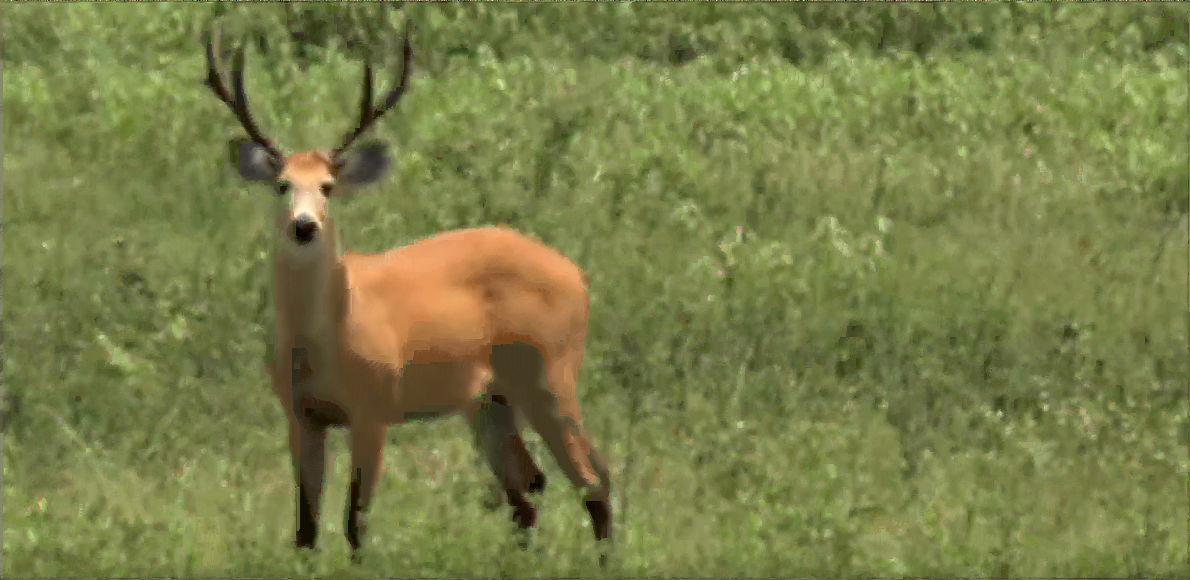
\includegraphics[width=.45\textwidth]{deer/deer.rec-src.p7.a0.5.w1190.propTrue.randTrue.iter1.png}\enskip
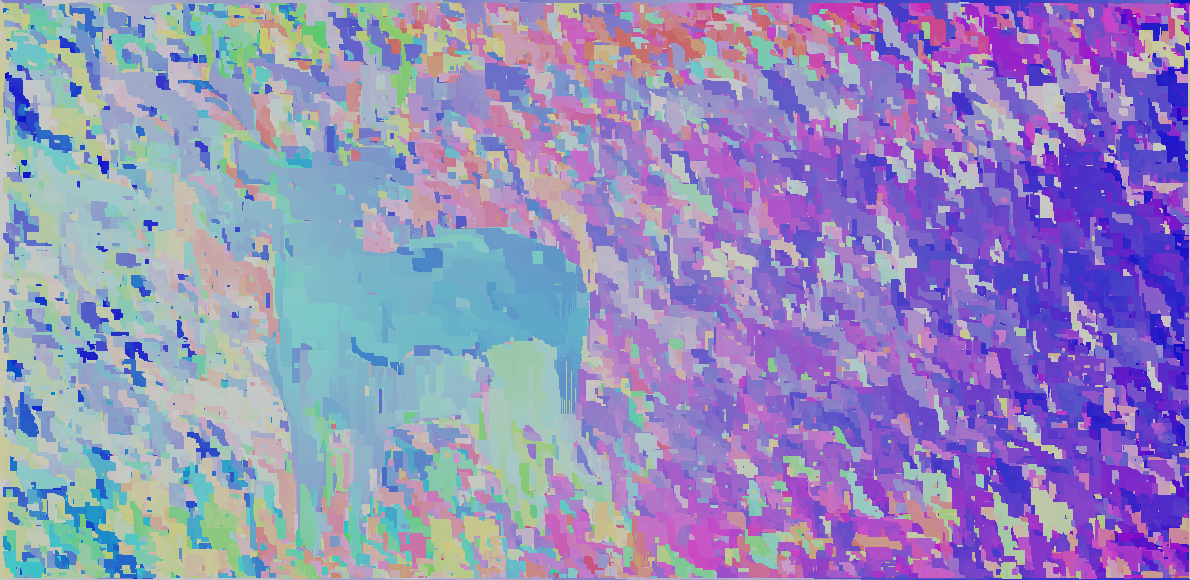
\includegraphics[width=.45\textwidth]{deer/deer.nnf-col.p7.a0.5.w1190.propTrue.randTrue.iter1.png}
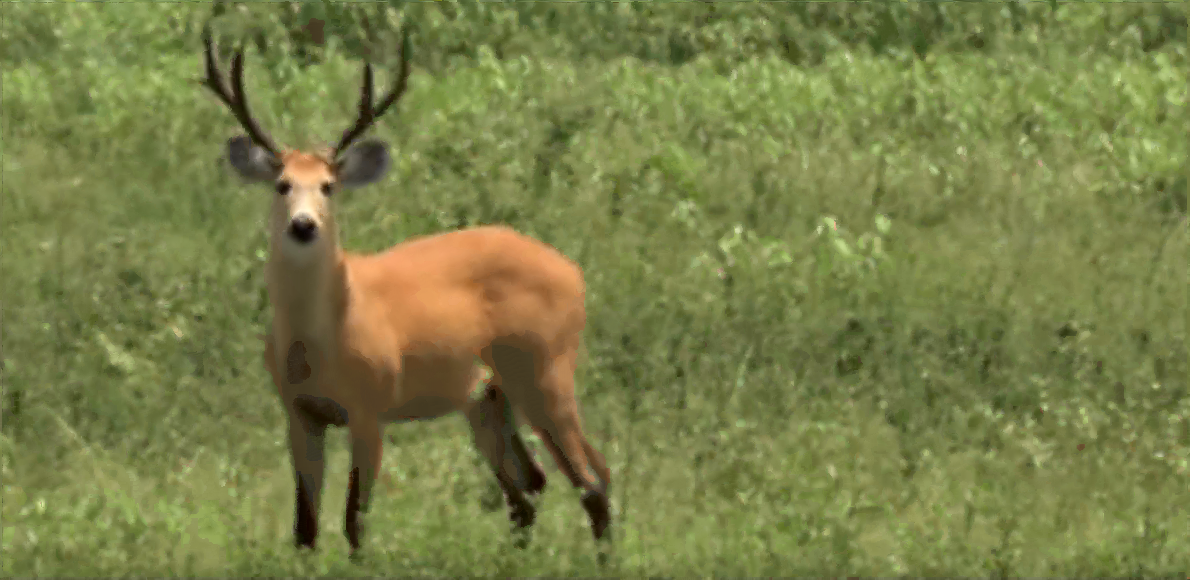
\includegraphics[width=.45\textwidth]{deer/deer.rec-src.p7.a0.5.w1190.propTrue.randTrue.iter2.png}\enskip
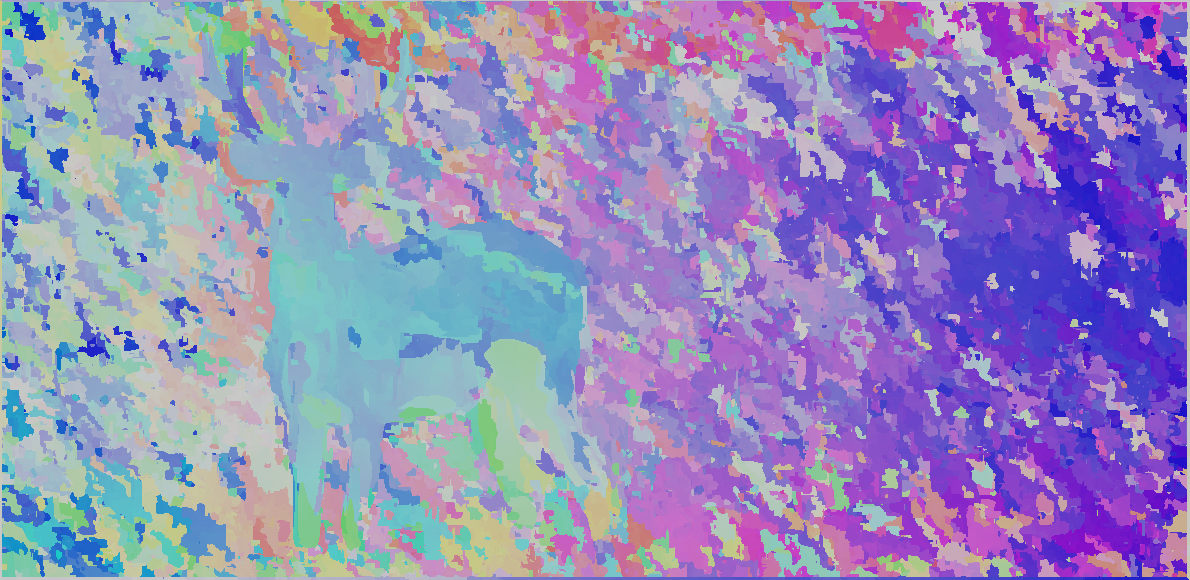
\includegraphics[width=.45\textwidth]{deer/deer.nnf-col.p7.a0.5.w1190.propTrue.randTrue.iter2.png}
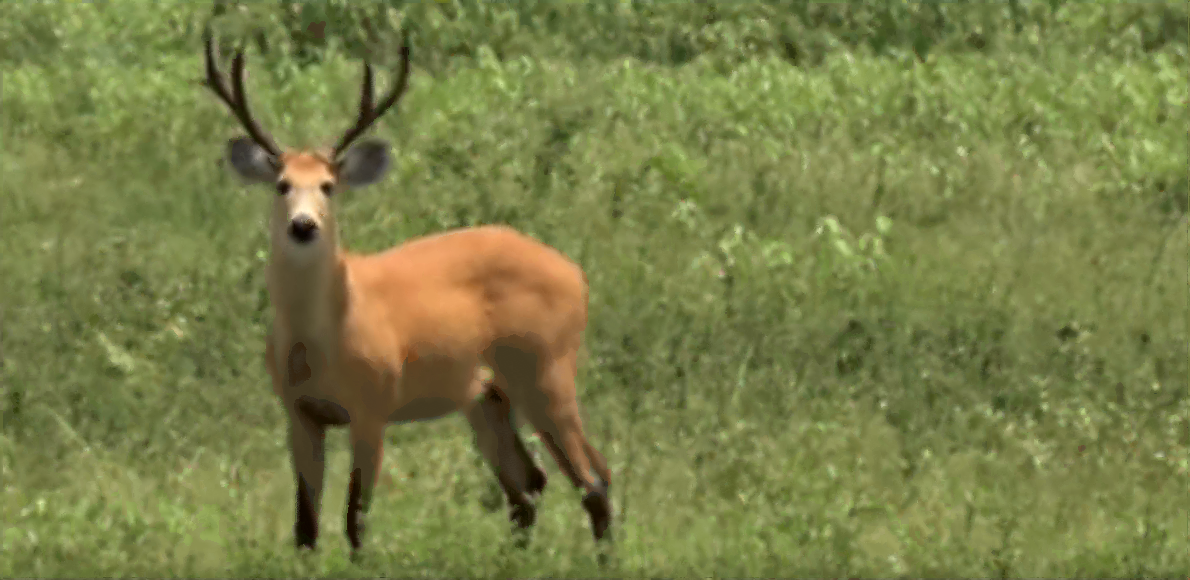
\includegraphics[width=.45\textwidth]{deer/deer.rec-src.p7.a0.5.w1190.propTrue.randTrue.iter3.png}\enskip
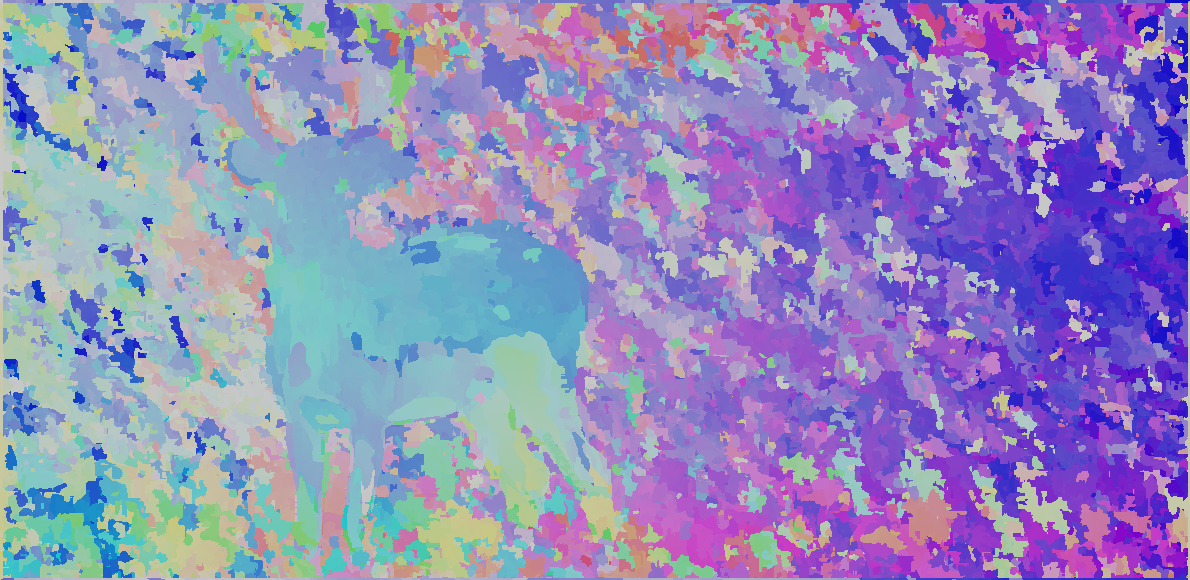
\includegraphics[width=.45\textwidth]{deer/deer.nnf-col.p7.a0.5.w1190.propTrue.randTrue.iter3.png}
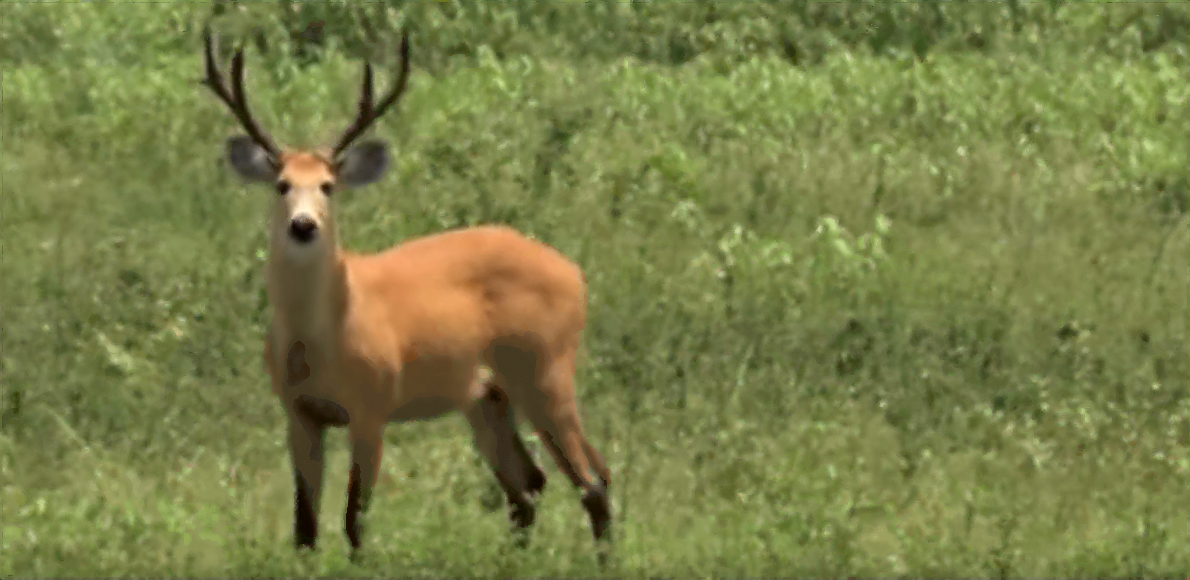
\includegraphics[width=.45\textwidth]{deer/deer.rec-src.p7.a0.5.w1190.propTrue.randTrue.iter4.png}\enskip
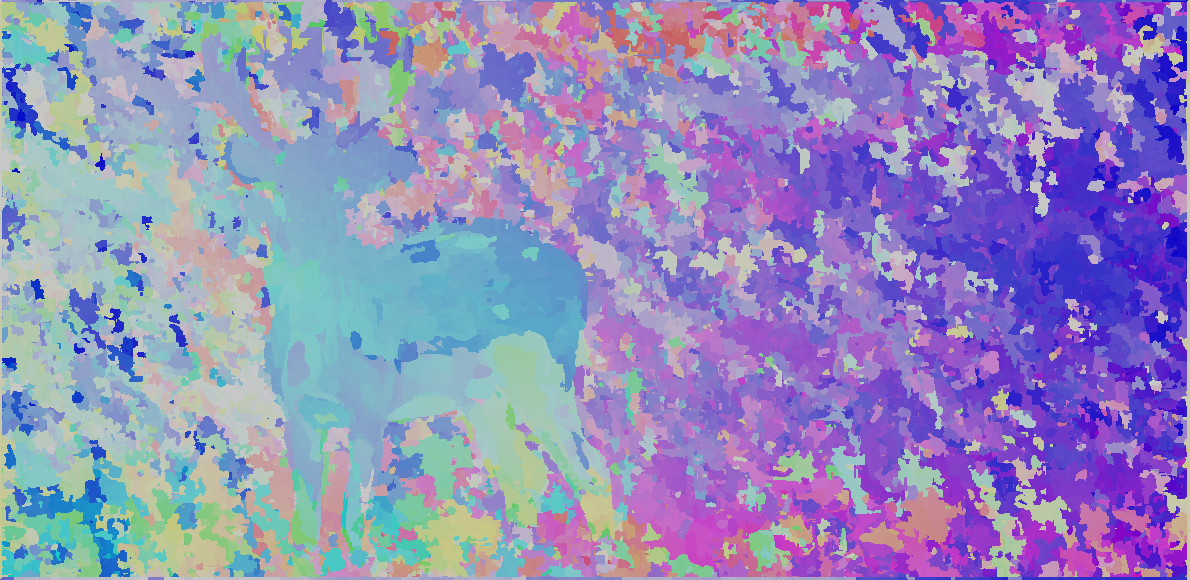
\includegraphics[width=.45\textwidth]{deer/deer.nnf-col.p7.a0.5.w1190.propTrue.randTrue.iter4.png}
\caption{deer}
\end{figure}

\begin{figure}[H]
\centering
\includegraphics[width=.45\textwidth]{jaguar/source.png}\enskip
\includegraphics[width=.45\textwidth]{jaguar/target.png}
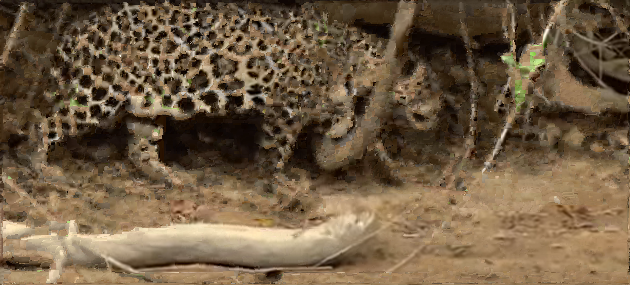
\includegraphics[width=.45\textwidth]{jaguar/jaguar.rec-src.p7.a0.5.w630.propTrue.randTrue.iter1.png}\enskip
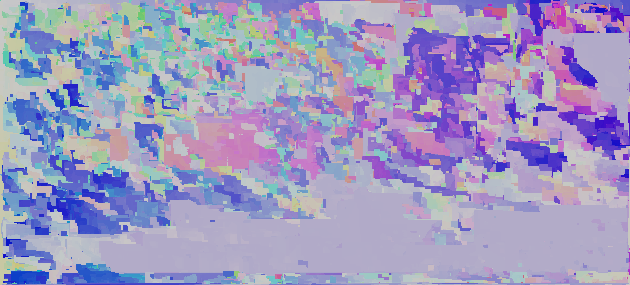
\includegraphics[width=.45\textwidth]{jaguar/jaguar.nnf-col.p7.a0.5.w630.propTrue.randTrue.iter1.png}
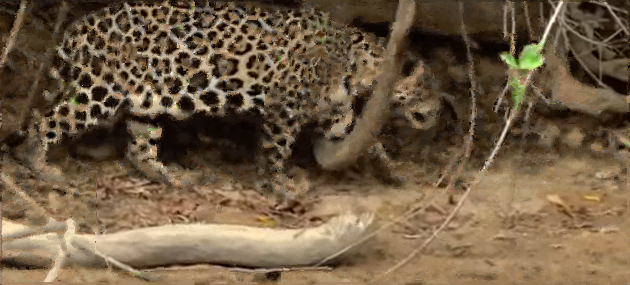
\includegraphics[width=.45\textwidth]{jaguar/jaguar.rec-src.p7.a0.5.w630.propTrue.randTrue.iter2.png}\enskip
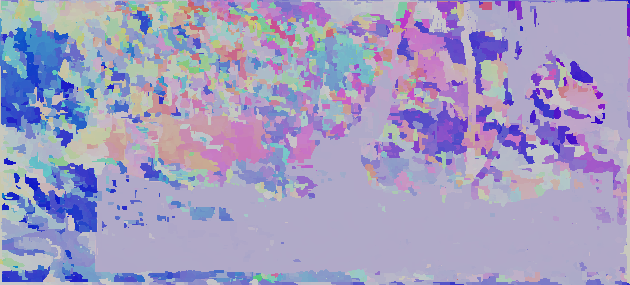
\includegraphics[width=.45\textwidth]{jaguar/jaguar.nnf-col.p7.a0.5.w630.propTrue.randTrue.iter2.png}
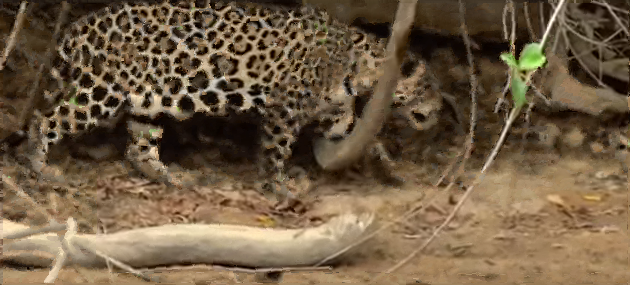
\includegraphics[width=.45\textwidth]{jaguar/jaguar.rec-src.p7.a0.5.w630.propTrue.randTrue.iter3.png}\enskip
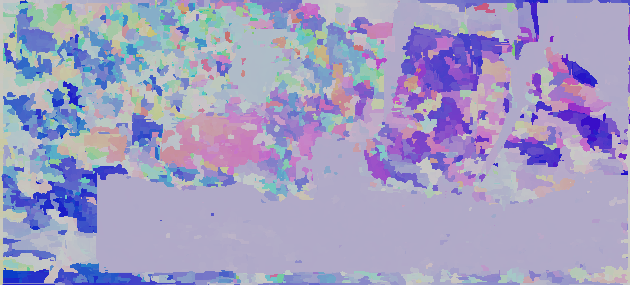
\includegraphics[width=.45\textwidth]{jaguar/jaguar.nnf-col.p7.a0.5.w630.propTrue.randTrue.iter3.png}
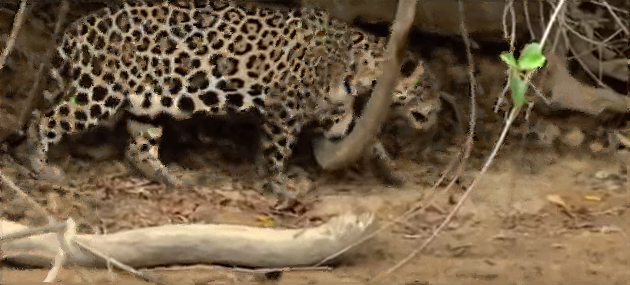
\includegraphics[width=.45\textwidth]{jaguar/jaguar.rec-src.p7.a0.5.w630.propTrue.randTrue.iter4.png}\enskip
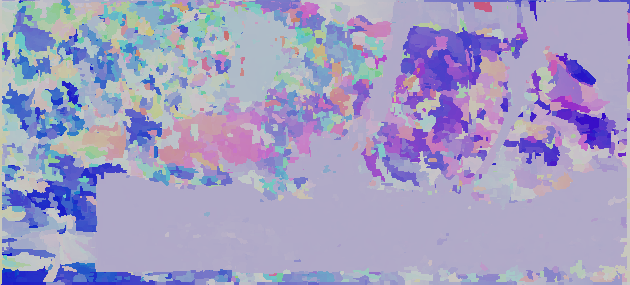
\includegraphics[width=.45\textwidth]{jaguar/jaguar.nnf-col.p7.a0.5.w630.propTrue.randTrue.iter4.png}
\caption{jaguar}
\end{figure}

\begin{figure}[H]
\centering
\includegraphics[width=.45\textwidth]{jaguar2/source.png}\enskip
\includegraphics[width=.45\textwidth]{jaguar2/target.png}
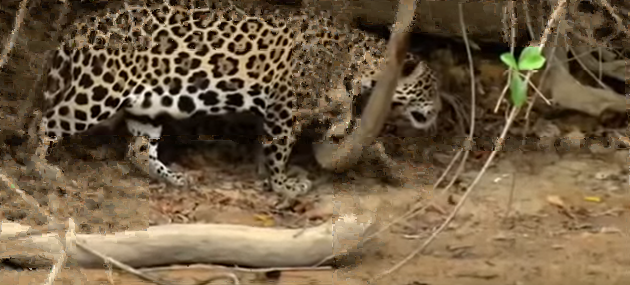
\includegraphics[width=.45\textwidth]{jaguar2/jaguar2.rec-src.p7.a0.5.w630.propTrue.randTrue.iter1.png}\enskip

\includegraphics[width=.45\textwidth]{jaguar2/jaguar2.nnf-col.p7.a0.5.w630.propTrue.randTrue.iter1.png}
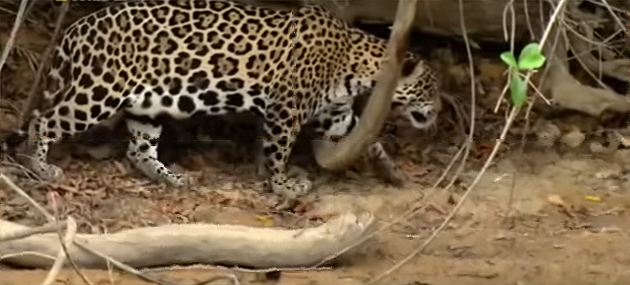
\includegraphics[width=.45\textwidth]{jaguar2/jaguar2.rec-src.p7.a0.5.w630.propTrue.randTrue.iter2.png}\enskip

\includegraphics[width=.45\textwidth]{jaguar2/jaguar2.nnf-col.p7.a0.5.w630.propTrue.randTrue.iter2.png}
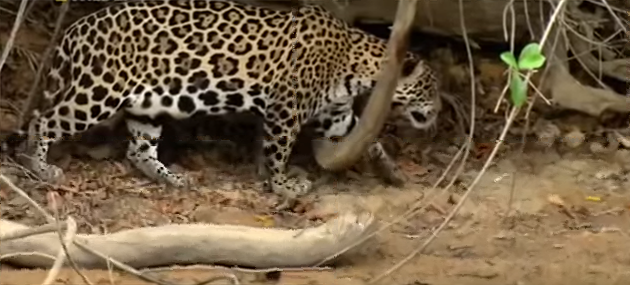
\includegraphics[width=.45\textwidth]{jaguar2/jaguar2.rec-src.p7.a0.5.w630.propTrue.randTrue.iter3.png}\enskip

\includegraphics[width=.45\textwidth]{jaguar2/jaguar2.nnf-col.p7.a0.5.w630.propTrue.randTrue.iter3.png}
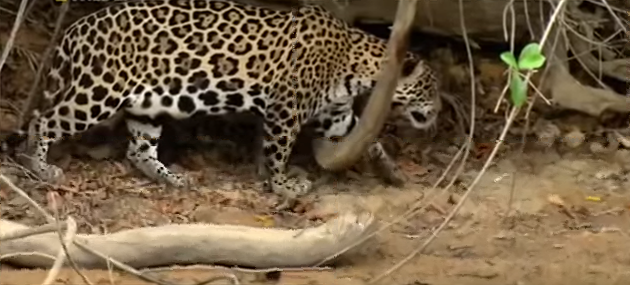
\includegraphics[width=.45\textwidth]{jaguar2/jaguar2.rec-src.p7.a0.5.w630.propTrue.randTrue.iter4.png}\enskip
\includegraphics[width=.45\textwidth]{jaguar2/jaguar2.nnf-col.p7.a0.5.w630.propTrue.randTrue.iter4.png}
\caption{jaguar2}
\end{figure}

\begin{figure}[H]
\centering
\includegraphics[width=.45\textwidth]{jaguar3/source.png}\enskip
\includegraphics[width=.45\textwidth]{jaguar3/target.png}
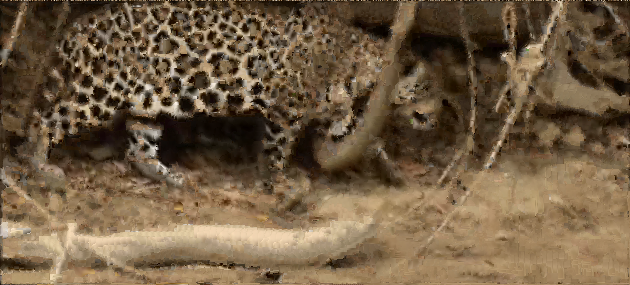
\includegraphics[width=.45\textwidth]{jaguar3/jaguar3.rec-src.p7.a0.5.w630.propTrue.randTrue.iter1.png}\enskip
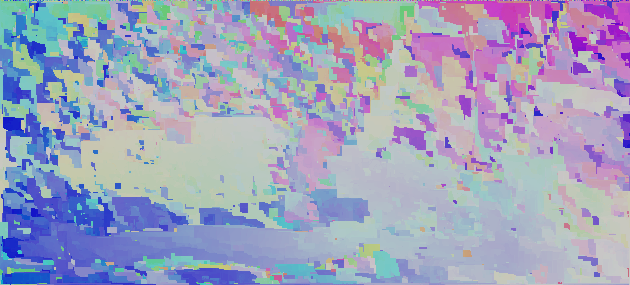
\includegraphics[width=.45\textwidth]{jaguar3/jaguar3.nnf-col.p7.a0.5.w630.propTrue.randTrue.iter1.png}
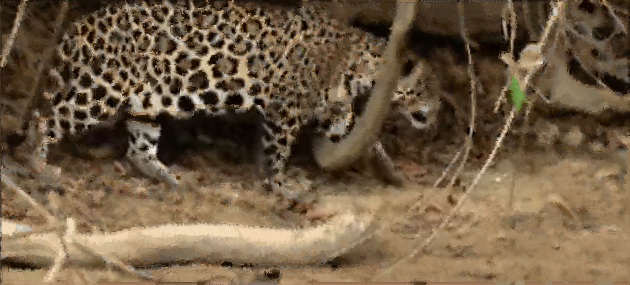
\includegraphics[width=.45\textwidth]{jaguar3/jaguar3.rec-src.p7.a0.5.w630.propTrue.randTrue.iter2.png}\enskip
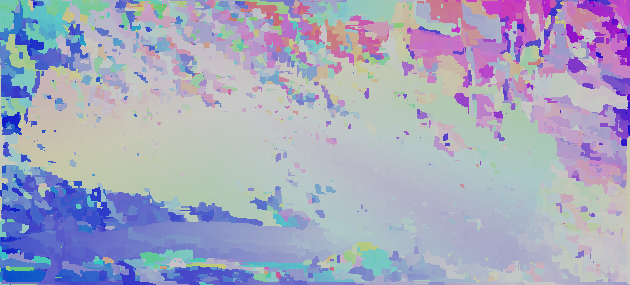
\includegraphics[width=.45\textwidth]{jaguar3/jaguar3.nnf-col.p7.a0.5.w630.propTrue.randTrue.iter2.png}
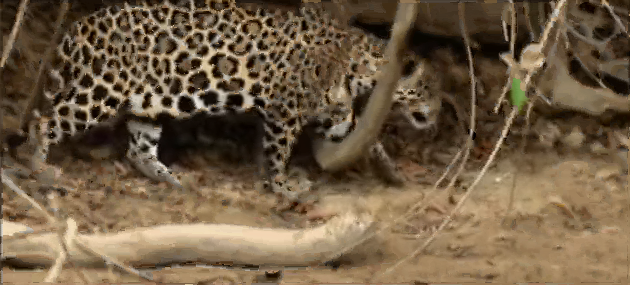
\includegraphics[width=.45\textwidth]{jaguar3/jaguar3.rec-src.p7.a0.5.w630.propTrue.randTrue.iter3.png}\enskip
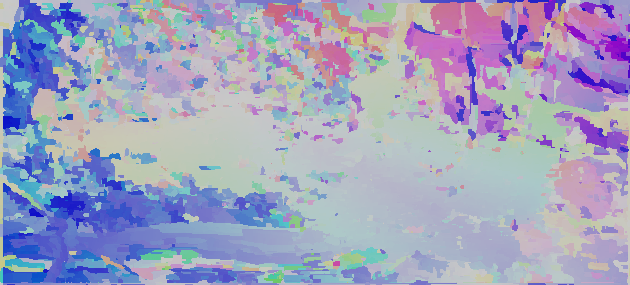
\includegraphics[width=.45\textwidth]{jaguar3/jaguar3.nnf-col.p7.a0.5.w630.propTrue.randTrue.iter3.png}
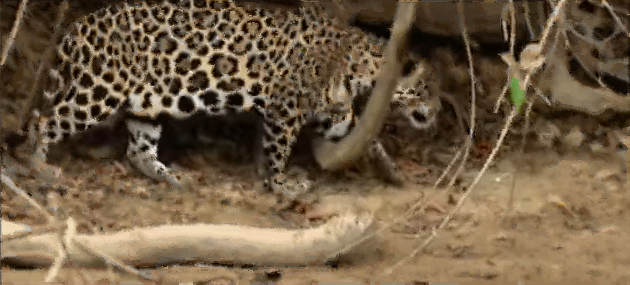
\includegraphics[width=.45\textwidth]{jaguar3/jaguar3.rec-src.p7.a0.5.w630.propTrue.randTrue.iter4.png}\enskip
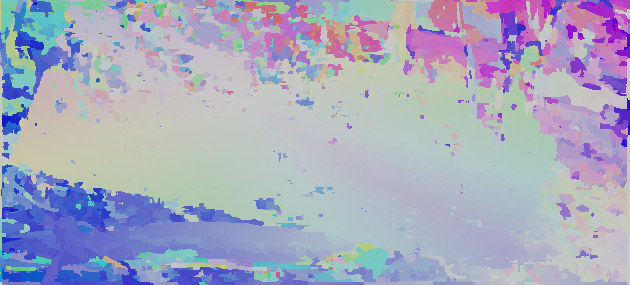
\includegraphics[width=.45\textwidth]{jaguar3/jaguar3.nnf-col.p7.a0.5.w630.propTrue.randTrue.iter4.png}
\caption{jaguar3}
\end{figure}

\begin{figure}[H]
\centering
\includegraphics[width=.4\textwidth]{spiderman/source.png}\enskip
\includegraphics[width=.4\textwidth]{spiderman/target.png}
\includegraphics[width=.4\textwidth]{spiderman/spiderman.rec-src.p7.a0.5.w1504.propTrue.randTrue.iter1.png}\enskip
\includegraphics[width=.4\textwidth]{spiderman/spiderman.nnf-col.p7.a0.5.w1504.propTrue.randTrue.iter1.png}
\includegraphics[width=.4\textwidth]{spiderman/spiderman.rec-src.p7.a0.5.w1504.propTrue.randTrue.iter2.png}\enskip
\includegraphics[width=.4\textwidth]{spiderman/spiderman.nnf-col.p7.a0.5.w1504.propTrue.randTrue.iter2.png}
\includegraphics[width=.4\textwidth]{spiderman/spiderman.rec-src.p7.a0.5.w1504.propTrue.randTrue.iter3.png}\enskip
\includegraphics[width=.4\textwidth]{spiderman/spiderman.nnf-col.p7.a0.5.w1504.propTrue.randTrue.iter3.png}
\includegraphics[width=.4\textwidth]{spiderman/spiderman.rec-src.p7.a0.5.w1504.propTrue.randTrue.iter4.png}\enskip
\includegraphics[width=.4\textwidth]{spiderman/spiderman.nnf-col.p7.a0.5.w1504.propTrue.randTrue.iter4.png}
\caption{spiderman}
\end{figure}

\begin{figure}[H]
\centering
\includegraphics[width=.4\textwidth]{woman/source.png}\enskip
\includegraphics[width=.4\textwidth]{woman/target.png}
\includegraphics[width=.4\textwidth]{woman/woman.rec-src.p7.a0.5.w1504.propTrue.randTrue.iter1.png}\enskip
\includegraphics[width=.4\textwidth]{woman/woman.nnf-col.p7.a0.5.w1504.propTrue.randTrue.iter1.png}
\includegraphics[width=.4\textwidth]{woman/woman.rec-src.p7.a0.5.w1504.propTrue.randTrue.iter2.png}\enskip
\includegraphics[width=.4\textwidth]{woman/woman.nnf-col.p7.a0.5.w1504.propTrue.randTrue.iter2.png}
\includegraphics[width=.4\textwidth]{woman/woman.rec-src.p7.a0.5.w1504.propTrue.randTrue.iter3.png}\enskip
\includegraphics[width=.4\textwidth]{woman/woman.nnf-col.p7.a0.5.w1504.propTrue.randTrue.iter3.png}
\includegraphics[width=.4\textwidth]{woman/woman.rec-src.p7.a0.5.w1504.propTrue.randTrue.iter4.png}\enskip
\includegraphics[width=.4\textwidth]{woman/woman.nnf-col.p7.a0.5.w1504.propTrue.randTrue.iter4.png}
\caption{actress}
\end{figure}

\end{document}